\chapter{Laser Interferometers for Gravitational-wave Detection}

We show in this chapter how a laser interferometer can detect
gravitational wave strain, and we present the basic design principles
of the LIGO detectors. We motivate the desire for higher laser power,
and introduce some of the details of the interferometer that are
relevant for later chapters. To reduce clutter, I do not specify the
polarization of the gravitational wave strain and use simply $h$ for
its symbol.


\section{Measuring Gravitational-wave Strain with Light}
Considering a simple Michelson interferometer consisting of a laser, a
beam splitter, and two end mirrors each a distance $L$ from the beam
splitter, one can understand intuitively why an interferometer can
detect gravitational waves. If an appropriately polarized
gravitational wave is present, it will stretch one arm and compress
the other. For two wave packets leaving the beam splitter at the same
time, each heading down a different arm, the roundtrip travel time for
the light traveling down the stretched arm is longer than that for the
light traveling down the compressed arm. For the stretched arm the
roundtrip travel time is:
\begin{equation}
t_{\mathrm{stretched}} = \frac{2 L}{c} \left( 1 + \frac{h}{2} \right),
\label{eq:trt+} 
\end{equation}
and for the compressed arm the roundtrip travel time is:
\begin{equation}
t_{\mathrm{compressed}} = \frac{2 L}{c} \left( 1 - \frac{h}{2} \right).
\label{eq:trt-} 
\end{equation}
A stationary clock at the beam splitter could, in principle, measure
the non-zero difference in arrival times, $\Delta t = 2Lh/c$, of the
two different wave packets.\footnote{It should be noted that $h$ is
  treated as a constant in Eqs. \ref{eq:trt+} and \ref{eq:trt-}. We
  use the approximation that the gravitational wave wavelength
  $\lambda_{gw}$ is much larger than the Michelson arm length
  $L$. This means that the temporal variation of $h(t)$ is negligible
  during the time it takes the photon to make its roundtrip.}

In practice we send a
continuous electromagnetic wave into the interferometer. The
difference in travel times turns into a difference in phase of
the beams returning to the beamsplitter:
\begin{equation}
\Delta \phi_{\mathrm{MICH}} = \omega \Delta t = \frac{2 L}{c} \omega h,
\label{eq:deltaphi}
\end{equation}
where $\omega$ is the angular frequency of the laser light. We now
introduce the modified Michelson interferometer used in LIGO, and in
this context continue the discussion of strain measurement and
sensitivity.

% reference to treatment as a wave, gauge-independent quantity.



\section{Power-recycled Fabry-P\'{e}rot Michelson Interferometers} 
The LIGO detector configuration is a power-recycled Fabry-P\'{e}rot
Michelson laser interferometer as depicted in
Fig.~\ref{fig:IFOschematic}. A beam splitter (BS) directs 1064~nm
light from a diode-pumped, power amplified, and intensity and
frequency stabilized Nd:YAG laser to the Fabry-P\'{e}rot arms, which
are made of an input test mass mirror (ITM) and an end test mass
mirror (ETM). Both arms are of length $L \approx 4 \text{ km}$ and are
set to maintain nearly perfect destructive interference of the
recombined light at the anti-symmetric (AS) port, where a
photodetector is placed to measure any change in power. A power
recycling mirror (RM) at the symmetric port directs the
constructively-interfered light back into the interferometer.

\begin{figure}
\begin{centering}
\includegraphics{figures/IFOsimple_thesis.pdf}
\caption[Power-recycled Fabry-P\'{e}rot Michelson laser
interferometer]{Power-recycled Fabry-P\'{e}rot Michelson laser
  interferometer.}
\label{fig:IFOschematic}
\end{centering}
\end{figure}

The Fabry-P\'{e}rot arms are a modification to the Michelson that
increases the change in phase measured at the AS port compared to that
for a simple Michelson. Rather than make a single roundtrip down each
arm, the light is trapped by the Fabry-P\'{e}rot cavity, experiencing many
roundtrips before returning to the beam splitter and interfering with
the light from the other arm. The effect is that Eq.~\ref{eq:deltaphi}
for the Fabry-P\'{e}rot Michelson includes a frequency-dependent phase
gain factor, $g_{\phi}(f)$:
\begin{equation}
\Delta \phi = \frac{2 L}{c} \omega g_{\phi}(f) h.
%\Delta \phi = \frac{2 L}{c} \omega g_{\phi}(f) \Delta h.
\label{eq:deltaphi}
\end{equation}
For Enhanced LIGO, $g_{\phi} = 137$ at DC and falls off as $1/f$ after
85~Hz due to the storage time of the light in the arm cavities.

The power recycling mirror is a modification to the Michelson
interferometer that increases the circulating power by a factor of
$g_{cr}^2 \approx 40$. Details are in Appendix~\ref{sec:impedance}.


\subsection{DC readout}
\label{sec:DCreadout}
The gravitational wave readout in Enhanced LIGO was not operated
precisely at the dark fringe at the AS port. Instead, it used a small
offset from the quadratic minimum so that small changes in phase
linearly produce power changes as is depicted in
Figure~\ref{fig:DCreadout}. The offset used was $\phi_0 \approx 6
\times 10^{-5}$~rad; the technique is a form of homodyne detection
called DC readout~\cite{TobinThesis}.

With a DC offset, the electric field at the AS port is $E_{AS} =
E_{BS}\sin{(\phi_0 + \Delta\phi)}$. Squaring the electric field and
expanding about $\phi_0$, we determine the power incident on the
photodetector, $P_{AS}$:
\begin{align}
P_{AS} &= P_{BS} \sin^2{(\phi_0 + \Delta\phi)} \\
% &\approx P_{BS}\sin^2{(\phi_0)} + 2P_{BS}\sin{(\phi_0)}\cos{(\phi_0)}\Delta\phi
 &\approx P_{BS}\sin^2{(\phi_0)} + 2P_{BS}\phi_0\Delta\phi
\end{align}
The first term on the right hand side of the expanded $P_{AS}$ is the
DC power due to the static offset from the fringe. The second term on
the right hand side describes how a change in phase at the beam
splitter is converted to a change in power:
\begin{equation}
\frac{d P_{AS}}{d \phi_{BS}} =2 P_{BS} \phi_0 
%\mathrm{phase\ optical\ gain} = \frac{4 L}{c} P_{BS} \phi_0 \omega \phi_g(f) h.
\label{eq:dP_dphi}
\end{equation}
This relationship is linear and proportional to the power at the beam
splitter. Throughout this dissertation, when we refer to signals
falling in a \emph{linear regime}, we mean that they are small enough
to be well modeled by a tangent to the actual response, just as for
the case described here regarding small phase signals.

\begin{figure}
\begin{centering}
\includegraphics{figures/DCreadout.pdf}
\caption[The DC readout dark fringe]{The DC readout dark fringe. The
  AS port is not kept at the dark fringe, but is slightly offset by
  $\phi_0$. Changes in phase at the beam splitter are a linear
  function of power.}
\label{fig:DCreadout}
\end{centering}
\end{figure}



\subsection{DARM}
The differential arm length (commonly known as DARM) is of central interest. This
is the length degree of freedom affected by gravitational waves. It is
defined as
\begin{equation}
\mathrm{DARM} := L_- := L_x - L_y
\end{equation}
where $L_x$ and $L_y$ are the lengths of the $x$-arm and $y$-arm,
respectively. When there is no gravitational wave, $L_-=0$, but in the
presence of a gravitational wave, the DARM signal is:
\begin{equation}
L_- = Lh
\label{eq:DARMandh}
\end{equation}
We see that $L$ is the conversion factor between GW strain and DARM.



\subsection{DARM Optical Gain}
The DARM optical gain tells how displacement is converted to power at
the AS port and has units of Watts per meter. Combining
Eqs.~\ref{eq:deltaphi}, \ref{eq:dP_dphi}, and \ref{eq:DARMandh}, the
DARM optical gain of the LIGO interferometer with DC readout is:
\begin{equation}
\frac{d P_{AS}}{dL_-} = \frac{4}{c} P_{BS} \phi_0 \omega g_{\phi}.
\label{eq:opticalgain}
\end{equation}




\section{Signal Versus Noise} 
From Eq.~\ref{eq:opticalgain} we see three fundamental
ways to increase the DARM optical gain and therefore produce more
power at the AS port for a given GW strain:
\begin{enumerate}
\item Make the arms longer. \vspace{-10 pt}
\item Increase the power at the beamsplitter. \vspace{-10 pt}
\item Increase the phase gain of the Fabry-P\'{e}rot arms.
\end{enumerate}
Our ability to detect gravitational wave strain is
dependent not only on the optical gain, but also on the detector noises,
which will mask a weak GW signal. No matter how large a
signal one might have, it won't be found confidently, or at all, if
there is too much noise. 


\subsection{Noises}
The sources of noise which contaminate the detector's output can be 
generally grouped into two categories:
\begin{enumerate}
\item displacement noise \vspace{-10 pt}
\item sensing noise
\end{enumerate}
Displacement noises are those that create real motion of the mirrors
(including the DARM degree of freedom), while sensing noises are those
that arise in the process of measuring the electric field at the 
detector's output.

The primary displacement noise that plagues terrestrial laser
interferometers is motion of the ground, i.e. seismic noise.  Thermal
motion of the mirrors and their suspensions are another source of
displacement noise. 

%% \begin{equation}
%% F(f) = \sqrt{4k_BTb(f)},
%% \end{equation}
%% where $k_B$ is Boltzmann's constant, $T$ is temperature, and $b$ is
%% the mirror's dissipation.

%%  With improvements in seismic isolation, future
%% detectors will be limited at low frequency by photon radiation pressure
%% noise.

The primary sensing noises are electronics (`dark') noise (due to
thermal noise in resistors and electronic amplifiers), and shot
noise, which arises from the Poisson statistics of photon arrival
at the photodetector. Shot noise appears as a
fluctuating power with amplitude spectral density:
\begin{equation}
P_{SN} = \sqrt{2 P h_p \nu}
\label{eq:shotnoise}
\end{equation}
where $P$ is the mean power on the photodiode, $h_p$ is Planck's
constant, and $\nu$ is the frequency of the incident light. Shot noise
is spectrally white.  The detector electronics are typically designed
so that electronics noise is never limiting.

% (with units of W/$\sqrt{\mathrm{Hz}}$) 
\subsection{Noise Floor}
The detector's noise floor is limited by seismic noise below 40~Hz and
by shot noise above 200~Hz.   In general we endeavor to push the noise floor down as far as possible
so that any underlying GW signals will be revealed.  Whether
limited by displacement noise or by sensing noise, the noise floor,
calibrated in strain, can be lowered by increasing the length of the
arms, which acts as the conversion from strain to effective displacement
(Eq.~\ref{eq:DARMandh}).
Further improvements require considering the noise
sources individually.

\subsubsection{Displacement noise floor} 
At frequencies where the noise floor is limited by displacement noise,
simply increasing the DARM optical gain will not help. The mirror
displacements, whether due to gravitational waves or due to ground
motion, are converted into power at the AS port in the exact same
way.   Reduction of displacement noises mainly relies on the development
of more sophisticated seismic isolation systems and mirror suspension
arrangements.

% You should make the point that improvements in the displacement noise
% floor are only linear in the arm length, whereas each additional stage
% of seismic isolation can potentially reduce the displacement noise 
% by 1/f^2.  Make the point that we already have 1/f^n attenuation.  Also, 
% of course, increasing the LIGO arm lengths is not actually an option.

\subsubsection{Sensing noise floor}
The noise floor due to sensing noise is improved by increasing the
optical gain. 
In particular, the contribution due to shot noise  may be found by 
dividing the shot noise amplitude spectral density by the optical gain,
\begin{equation}
h_{shot} = \sqrt{\frac{h_p}{2 P_{BS} \nu}} \frac{c}{4 \pi L g_{\phi}}
\quad \text{W}/\sqrt{\text{Hz}}.
\label{eq:SNL}
\end{equation}

Here we see that the shot noise limit (calibrated in effective strain)
drops with increases in the optical gain. 
Increasing the power in the interferometer improves the shot noise limit
because the optical gain increases more quickly ( $\propto
P_{BS}$, see Eq.~\ref{eq:opticalgain}) than the shot noise amplitude
(which goes like $\sqrt{P_{BS}}$, assuming the DARM offset is held
constant).

% Increasing the power at the beam splitter and therefore lowering the
% noise floor above 200~Hz is a goal of this work. The power at the BS
% is dependent on several quantities:
% \begin{itemize}
% \item input power \vspace{-10 pt}
% \item input efficiency \vspace{-10 pt}
% \item power reycling gain
% \end{itemize}
% Improving the Input Optics allows for greater input power and better
% input efficiency. Improving the Angular Sensing and Control allows for
% greater input power and better power recycling gain.



% \section{DC readout / more laser power}
% Increasing the laser power in the interferometer is a 

% Shot noise is a Poissonian process: the average number of photons
% striking a detector, $\left<x\right>$, is equal to the variance of the
% mean number of photons, $\left<x^2\right> - \left<x\right>^2$, from a
% given chunk of time $\tau$ to another. For large $\left<x\right>$, the
% distribution becomes Gaussian, but the mean and variance are still
% equivalent. Based on this property and Parseval's theorem, the power
% on a detector due to shot noise is:


%A summary of the noise budget is shown in Fig. \ref{fig:NB}.

% \begin{figure}
% \begin{centering}
% %\includegraphics[width=0.8\textwidth]{figures/.pdf}
% \caption[LIGO noise budget]{Noise budget place holder.}
% \label{fig:NB}
% \end{centering}
% \end{figure}




\section{Controlling the Interferometer}
The ability of the interferometer to operate as described above
requires that the many interferometer
cavities be held on resonance. The motion
of the mirrors in the absence of control is much too large 
--on the order of 1\micron, a full wavelength!--to maintain resonance.
The motion of the interferometer mirrors must therefore be controlled.
A feedback control system is implemented to hold the system sufficiently
near (for DARM, within $\sim 10^{-13}$ m) the intended operating point so that the response to residual
deviations remains linear.  (Calibration of the detector must take
into account the action of the control system.)

% Since the strain sensitivity is determined
% by mathematically undoing the (carefully measured) effect of the
% control system on DARM, control does not directly improve the strain
% sensitivity. The purpose length control does serves is to make the
% strain measurement possible. For other degrees of freedom, such as
% angular motion, only the controlled residual matters ..  Control,
% however, introduces noise so there is a fine balance that must be
% found between too much and too little control.

% Design considerations for the control loops include how much motion at
% what frequencies can be tolerated, and the signal to noise ratio of
% the motion sensor.


% \subsection{RF Sidebands}
% Phase modulation multiplies carrier light with field
% $E_0e^{i\omega t}$ by $e^{i \Gamma \sin{(\Omega t)}}$, where $\Gamma$
% is the modulation index and $\Omega$ is the frequency of the phase
% modulation. Using the Jacobi-Anger expression,
% \begin{equation}
% e^{i z \sin{\theta}} = \sum_{n=-\infty}^{\infty} J_n(z) e^{i n \theta},
% \end{equation}
% where $J_n$ are the Bessel functions, we can write the first few terms
% (n = 0, 1, -1) of the phase-modulated field:
% \begin{equation}
% E_{modulated} = E_0 J_0(\Gamma) e^{i\omega t} + E_0 J_1(\Gamma)
% e^{i(\omega + \Omega) t} + E_0 J_{-1}(\Gamma)
% e^{i(\omega - \Omega) t} + ...
% \end{equation}
% We see that both an upper and lower primary sideband are created, with
% frequencies $\omega + \Omega$ and $\omega - \Omega$. Phase modulation
% does produce an infinite number of sidebands, yet the amplitude of the
% Bessel function decays rapidly with higher $|n|$, so only this first
% set of sidebands are significant.




\subsection{Digital Control in LIGO}
Although the interferometer is an analog instrument, it is interfaced
through a digital control system. The analog sensor signals are sent
through analog-to-digital converters (ADCs), digitally filtered, and
then sent through digital-to-analog converters (DACs) before returning
to the interferometer's actuators as control signals. The 
digital control system allows complex filters to be implemented and
tuned from a comfortable control-room environment.

The various LIGO subsystems operate at different sample rates.  The
length sensing and control (LSC) subsystem, which measures and
controls DARM, in addition to other length degrees of freedom,
operates at 16384 samples/second, while the angular sensing and
control (ASC) sytem, which maintains mirror alignment, operates at
2048 samples/second.  In addition to the all-important DARM channel,
many other auxiliary data streams are permanently recorded.

% There are a select few control systems that remain completely analog, like
% the laser intensity stabilization servo (ISS). When the frequencies of
% interest extend beyond several tens of thousands of Hz, the use of
% computers becomes impractical.




\subsection{Mirror Suspension and Actuation}
\label{sec:suspension}
The primary interferometer optics are suspended in vacuum so that they
act like free masses at the frequencies in the GW detection band, and
so that they are isolated from ground motion. Each mirror is hung from
a single wire that loops around the bottom of the barrel of the mirror
as shown in Fig.~\ref{fig:suspension}. Stand-offs glued just above the
mirror's center of mass on both sides of the barrel mark the final
point of contact of the wire with the mirror, and both ends of the
wire are clamped to the top of a suspension cage.

\begin{figure}
\begin{centering}
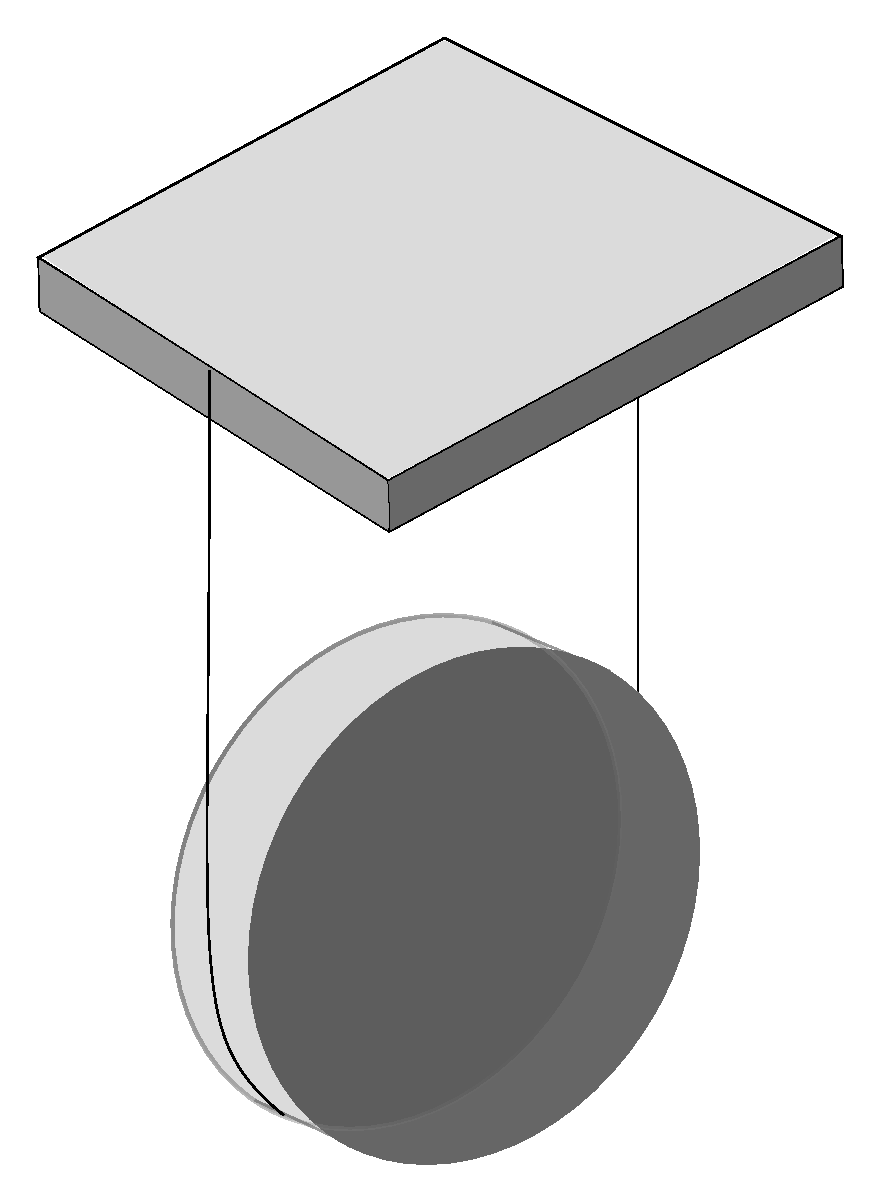
\includegraphics[width=0.3\textwidth]{/Users/kate/kate-thesis/figures/suspension.pdf}
\caption[Sketch of a LIGO suspension]{Sketch of a LIGO suspension.}
\label{fig:suspension}
\end{centering}
\end{figure}

Each mirror is equipped with four optical sensor and electro-magnetic
(OSEM) actuators for rough sensing and fine control of the mirror position and orientation. Magnets arranged
to form the four corners of a square are glued on the mirror's back
surface which are enveloped by the OSEM solenoid coil. 
The currents through each coil may be driven independently.
Length control of the
cavities, for instance, sends current of the same magnitude through
each coil on a given mirror to provide a piston force for changing the
mirror's position.  OSEM sensing is accomplished through simple shadow
sensors.

To avoid thermal noise, the mirror suspensions are designed to minimize 
dissipation.
Damping for the large optics is achieved through
electronic servos.  Motion of the optics corresponding to a change
in cavity length is damped using simple velocity damping servoes
implemented using the OSEM sensors and actuators, while angular
motion is sensed via optical levers.
The optical levers provide velocity damping\footnote{
The open loop transfer function of the optical lever
servo is described in Appendix~\ref{sec:oplevOLG}.
} only (no DC control) between
0.2~Hz and 2~Hz. 

% The suspensions are AC damped at all times for each of the large
% optics through optical lever witnesses. Keeping the mirrors quiet
% enough with respect to their local ground is necessary to allow for
% the initial locking of the interferometer, so each suspended optic,
% small and large, is quieted by its OSEM signals during the initial
% locking stages. After the interferometer is locked, the angular OSEM
% feedback is turned off, and the position OSEM feedback remains.

\section{Summary}
The modified Michelson interferometer provides a robust foundation on
which to build a gravitational wave detector in which fluctuating
gravitational wave strains are transduced into measurable optical
power fluctuations.  For the interferometer to operate properly, the
mirrors positions and orientations must be controlled.  The noise
floor of the interferometer may be improved in the shot noise
dominated regime by increasing the laser power circulating in the
interferometer.  Increases in laser power, however, create several
challenges; two such challenges are addressed in this thesis: coping
with the higher power in the interferometer's Input Optics (Chapter 3)
and dealing with radiation pressure induced angular instabilities
caused by high power in the interferometer's arm cavities (Chapters 4,
5, and 6).
